\documentclass[12pt,a4paper]{article}
\usepackage{amsthm,amsfonts,amsmath,amscd,amssymb}
\usepackage{latexsym}
\usepackage{euscript}
%\usepackage{enumitem}
\usepackage{caption}
\usepackage{cite}
\usepackage{listings}
\usepackage[utf8]{inputenc}
\usepackage[english, ukrainian]{babel}
\usepackage{xcolor}
\usepackage{graphicx}
\definecolor{darkgreen}{HTML}{00A000}
\definecolor{darkblue}{HTML}{0000A0}
\definecolor{darkred}{HTML}{D00000}
\usepackage[colorlinks=true]{hyperref}%%%%%%%%%
\hypersetup{linkcolor=darkred, urlcolor=darkblue, citecolor=darkgreen}%%%%%%%%
\graphicspath{ {./images/} }
%%%%%%%%%%%%%%%%%%
\tolerance=9000
\textwidth=150mm %160mm%11pt
\textheight=237mm %245mm %196.5mm%11pt
\oddsidemargin=5mm
%\evensidemargin=25mm
\topmargin-10mm
%\addtolength{\topmargin}{.5in}


\makeatletter %%%%%%%%%%%%%

%%%%%%%%%%%%%%%% PAGESTYLES %%%%%%%%%%%%%%%%%%%%

\newcommand{\ps@diploma}{%
\renewcommand{\@oddfoot}{}
\renewcommand{\@evenfoot}{}
\renewcommand{\@evenhead}{\underline{\makebox[160mm][c]{\lower.5em%
       \hbox  to 160mm{\thepage\hfil \sl \leftmark  \hfil}}}}%
%       
\renewcommand{\@oddhead}{\underline{\makebox[160mm][c]{\lower.5em%
       \hbox to 160mm{\hfill\large\slshape \rightmark \hfil\thepage}}}}%
}%

%%%%%%%%%%%%%%%%% END PAGESTYLES %%%%%%%%%%%%%%%
%%%%%%%%%%%%%% SECTIONS %%%%%%%%%%%%%%%%%%%
\renewcommand{\@seccntformat}[1]{\csname the#1\endcsname. }
\renewcommand{\section}{\@startsection{section}{1}{18pt}{3.25ex plus 1ex minus 0.2ex}%
{1.5ex plus .2ex}{\bfseries\rmfamily\Large}}
\renewcommand{\subsection}{\@startsection{subsection}{2}{18pt}{3.25ex plus 1ex minus 0.2ex}%
{-1.5ex plus .2ex}{\bfseries\rmfamily\large}} 

%%%%%%%%%%%%%%%% END SECTIONS %%%%%%%%%%%%%%%%%%

\makeatother

%%%%%%%%%%%%%%% THEOREMS %%%%%%%%%%%%%%%%%%%%%%%%

\newtheoremstyle{myplain}
  {\topsep}   % ABOVESPACE
  {\topsep}   % BELOWSPACE
  {\itshape}  % BODYFONT
  {18pt}       % INDENT (empty value is the same as 0pt)
  {\bfseries\Large} % HEADFONT
  {.}         % HEADPUNCT
  {5pt plus 1pt minus 1pt} % HEADSPACE
  {}          % CUSTOM-HEAD-SPEC
  
%%%%%%%%%%%%%%%%%%%%%%%%%%%%%%%%%%%%%%%
\theoremstyle{myplain}
\newtheorem{theorem}{Theorem}[section]
%%%%%%%%%%%%%%% END THEOREMS %%%%%%%%%%%%%%


%%%%%%%%%%%% LISTING %%%%%%%%%%%%%%%%%%%
\lstset{language=Python}
\lstset{frame=lines}
\lstset{basicstyle=\normalsize}
\lstset{prebreak=\raisebox{-2ex}[0ex][0ex]{\ensuremath{\hookleftarrow}}}
\lstset{breaklines=true}
\captionsetup[lstlisting]{font=large}
%%%%%%%%%%%%%% END LISTING %%%%%%%%%%%%%%%

\pagestyle{diploma}

\renewcommand{\baselinestretch}{1.4}

\numberwithin{equation}{section}

\newcommand{\sgn}{\operatorname{sgn}}

\newcommand{\cov}{\operatorname{cov}}

\begin{document}

\selectlanguage{english}

\begin{center}
cover page
\end{center}

\newpage

\tableofcontents

\newpage

\listoffigures
\listoftables

\newpage

\section*{Abstract}

The qualification work extends the already published article \cite{MainPaper}, in which one can find forecasting analysis for the time series with different approaches, their efficiency and comparison of tested methods on the three given data sets (all datasets could be found here: https://www.kaggle.com/). The sets represent the information collected by call centres. In this article we analyse the same data with other known methods such as $ ARIMA $ (Autoregressive Integrated Moving Average) and Exponential Smoothing, to study their performance and compare them with the algorithms provided in the related article \cite{MainPaper}.

\selectlanguage{ukrainian}

\section*{Анотація}

Кваліфікаційна робота є розширенням вже опублікованої статті \cite{MainPaper}, в якій аналізуються різні підходи до вивчення часових рядів, їх ефективність та порівняння протестованих на трьох масивах даних (усі дані можуть бути знайдені тут: https://www.kaggle.com/). Масиви представлені інформацією, зібраною колл центрами. У цій статті ми аналізуємо ті ж самі дані використовуючи інші відомі методи такі як ARIMA (Autoregressive Integrated Moving Average) й експоненційне згладжування, вивчимо їх результати й порівняємо з алгоритмами зі статті \cite{MainPaper}.

\selectlanguage{english}

\newpage

\section{Introduction}

%Call centres are in need of predicting future calls intensity with one simple but still very important goal, they should manage their budgets. To do this they need to choose close to the optimal amount of workers because the labour cost takes a significant portion of call centre's expenses. In order to reduce the number of employees in any given time we have to accurately know how many of them will be needed. To estimate such number we need to forecast the number of the incoming/outcoming calls. So we conclude that to lower the expenses we should predict the number of calls.

Call centres require a method of predicting future calls intensity with one simple but very important goal, the management of costs. To do this they need to choose an optimal number of employees as labour costs take a significant proportion of a call centre's expenses. In order to reduce the number of employees required at any given time we have to accurately know how many employees will be needed.To estimate such number we need to forecast the number of the incoming/outgoing calls. So to lower expenses we need to predict or forecast the number of calls.

%Forecasting is a difficult job due to the natural inconsistency of human behaviour which leads to randomness in the data, but the first problem comes when you decide: "How you are going to analyse?". In our time there is a wide variety of the algorithms with their respectful advantages and downsides. Here we test two algorithms designed specially for forecasting purposes, and also well suited to capture repeated trend which can be clearly seen in the given data due to its nature.

Forecasting is a difficult task due to the natural inconsistency of human behaviour which in turn may lead to inconsistent or random data. The first problem arises when you need to decide: "How you are going to analyse?". Currently, there are a wide variety of the algorithms with their respectful advantages and downsides. Here we test two algorithms designed specially for forecasting purposes, and are also well suited to capture repeat trends which can be clearly seen in the given data due to its nature.

%The data sets are represented by saved on hourly basis amount of calls handled by call centres including night period when no one works, data were collected during long period of time different for each set but still good enough to see intra-day and intra-week seasonality patterns. The set shows no pattern which could be easily predicted with occasional spikes and weekends which probably can be predicted as the consequences of real life events but this is out of the scope of our article. Here we are more focused on checking if given algorithms are capable of forecasting with no additional information or preprocessing of the data.

The data sets are represented by saved "hourly basis" numbers of calls handled by call centres including night periods when no one works. Data is collected during long periods of time, different for each set but still good enough to see intra-day and intra-week seasonality patterns. The set shows no pattern which could be easily predicted with occasional spikes and weekends which probably can be predicted as the consequences of real life events but this is out of the scope of our article. Here we are more focused on checking if the given algorithms are capable of forecasting with no additional information or preprocessing of the data.

%Two different approaches will be used in this work. ARIMA is one of them, this algorithm is designed to fit the repeating time series with non-linear behaviour. Given method has three different input parameters which allow you to increase the complexity manually to affect the performance. The second approach is Exponential Smoothing, this algorithm is in fact part of the ARIMA with the particular coefficients.

Two different approaches will be used in this work. ARIMA is one of them. This algorithm is designed to fit the repeating time series with non-linear behaviour. This method has three different input parameters which allows you to increase the complexity manually to affect the performance. The second approach is Exponential Smoothing. This algorithm is in fact part of the ARIMA but with particular coefficients.

\section{The call center arrivals forecasting problem}

%Rise for the forecasting problem came after rapid development of the computers, because work with big amount of data requires many computations with high precision. We do not talk about the complex tasks but about enormous cost of each mistake. Such task could be given to entity with close to zero rate of the miscalculations and the computer is the one. Humanity are no match for the chips in terms of fast and accurate performance of the complex mathematical operations. With such power in hands people start to design elegant algorithms to solve previously unresolvable problems. Since the dawn of computer science many problems were resolved. But among many problems a prediction for the time series is one of the hardest. The goal is simple, by studying the past behaviour predict the future. Many books were written about this topic (Montgomery et al. (2008)\cite{MainBook}; Ibrahim et al. (2016)\cite{Ibrahim_2016}). More specific book about call canters also could be found (Gans et al. (2003)\cite{Gans_2003}; Aksin et al. (2007)\cite{Aksin_2007}).

The rise of forecasting problems became evident after the rapid development of computers, as working with large amounts of data requires many computations with high levels of precision. We do not talk about the complexity of such tasks but about enormous cost of errors. Such task could be given to an entity with close to zero rate of the miscalculations and the computer is designed specifically to do this. Human intervention is no match for "silicon" in terms of fast and accurate performance of complex mathematical operations. With such power in the hands of people, programmers  started to design elegant algorithms to solve previously unresolvable problems. Since the dawn of computer science many problems have been resolved in the same manner. But among many problems a prediction for the time series is one of the hardest. The goal is simple, by studying the past behaviour to predict the future. Many books were written about this topic (Montgomery et al. (2008)\cite{MainBook}; Ibrahim et al. (2016)\cite{Ibrahim_2016}). More specific book about call canters also could be found (Gans et al. (2003)\cite{Gans_2003}; Aksin et al. (2007)\cite{Aksin_2007}).

Review of the solution for the call center arrivals forecasting problem.

The incoming calls were modelled as a Poisson arrival process (Garnett et al., 2002 \cite{Garnett_2002}; Gans et al., 2003 \cite{Gans_2003}; Wallace and Whitt, 2005 \cite{Wallace_and_Whitt_2005})), by assuming a very large population of potential customers where calls are statistically independent low-probability events. Later it has been observed that call centres arrivals show a relevant overdispersion (see e.g., Jongbloed and Koole, 2001 \cite{Jongbloed_and_Koole_2001}; Steckley et al., 2005 \cite{Steckley_2005}; Aldor-Noiman et al., 2009 \cite{Aldor-Noiman_2009}).

A non-homogeneous Poisson process, with non-constant arrival rate which is a deterministic function of the time is one of two ways used to handle previous problems (Brown et al., 2005 \cite{Brown_2005}; Green et al., 2007 \cite{Green_2007}). And second way is a doubly stochastic Poisson process (Avramidis et al., 2004 \cite{Avramidis_2004}; Liao et al., 2012 \cite{Liao_2012}; Ibrahim and L'Ecuyer, 2013 \cite{Ibrahim_and_LEcuyer_2013}).

Now we logically come to \textit{autoregressive integrated moving average} (ARIMA) (e.g., Andrews and Cunningham, 1995 \cite{Andrews_and_Cunningham_1995}; Bianchi et al., 1998 \cite{Bianchi_1998}; Antipov and Meade, 2002 \cite{Antipov_and_Meade_2002}; Taylor, 2008 \cite{Taylor_2008}; Montgomery, 2008 \cite{MainBook}) and \textit{Exponential Smoothing} (e.g., Taylor, 2010 \cite{Taylor_2010}; Barrow and Kourentzes, 2018 \cite{SidePaperSN}; Montgomery, 2008 \cite{MainBook})

Next step will be \textit{neural networks} (NN) and \textit{machine learning} (ML) which studied in related to this work articles (Manno et al., 2020 \cite{MainPaper}; Barrow and Kourentzes, 2018 \cite{SidePaperSN}).

\section{Methods}

In this section we describe both algorithms.

\subsection{Time series}

A time series can be defined as the collection of numerical points, time ordered and equally spaced. A more general description could be found for the continuous time series, but for the scope of this study description above its the most accurate to describe given sets. Our data is a good example of the time series with the time frequency of one hour. Were the time interval at which data is collection is generally referred to as the time series frequency. The data for this study are the integers, which represent number of incoming calls, collected on hourly basis.
Time series analysis is a process of extracting meaningful statistical and other characteristics from the data. Time series forecast is a process of predicting future values based on previously observed.

\subsection{Autocorrelation Function (ACF)}

During the analysis session we want to built a prediction based on known data, so we assume that previous observations are to correlate somehow with future results but we don't know how. To estimate this influence we use Autocorrelation Function (ACF).

ACF is a function that gives a map between lag, how far correlated objects apart, and correlation of this objects. In our case, lag is number of hours prior to observation and object is a number of calls during the observations. 

Since dataset used in this study similar with regard ACF we show only results for the ACD data set in Figure 1.
\begin{figure}
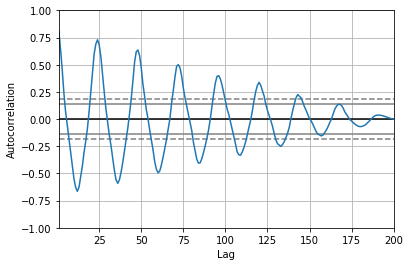
\includegraphics[scale=1]{ACD_ACF_plot}
\caption{The Autocorrelation Function plot for an ACD data set.}
\end{figure}
As we can see high correlation coefficient occurs every 24 hour period. Because of that, later we use this number as parameter for one of our prediction algorithms. Plot and results were obtained using following code:

\renewcommand{\lstlistingname}{Block of code}
\lstset{caption={ARIMA realisation.}}
\begin{lstlisting}
import pandas as pd

test = Data_frame_Calls_training.iloc[:200,:]
pd.plotting.autocorrelation_plot(test)
plt.show()
\end{lstlisting}

where $Data\_frame\_Calls\_training$ is a training set for ACD dataset.

\subsection{Exponential Smoothing methods}

A data set could be described as consisting of two distinct components: signal and noise. To predict the behaviour of data it is useful primarily to find data's signal which represents the process's intrinsic dynamics for collected information. Smoothing can be seen as a technique to separate the signal and the noise with the goal to give some estimation for the signal. In Figure 2 we give some examples for this process.

For forecasting both signal and noise plays major role because the goal is to predict results as accurately as it possible. If we discover signal it helps us to understand how data behaves but noise is a hidden change which makes processes natural. Mostly we assume that noise part has mean 0, to be uncorrelated and with constant variance. Such assumption highlights randomness in noise part and its natural occurrence.

\begin{figure}
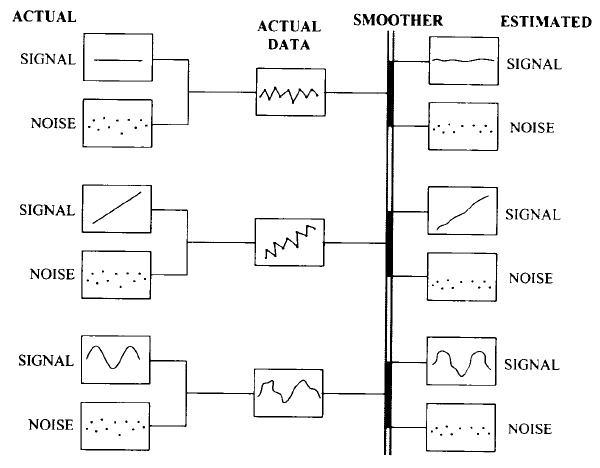
\includegraphics[scale=0.9]{Process_of_smoothing}
\caption{The process of smoothing a data set.}
\end{figure}

Exponential Smoothing is a technique for the data approximation. It could be performed simply by using following formula:
\begin{equation}
\tilde{y}_t = \lambda y_t + (1 - \lambda)\tilde{y}_{t - 1}.
\end{equation}

By re-writing this formula and adding a concept of prediction error which will be denote as $ e_t $, we now can forecast future values:
\begin{equation}
\tilde{y}_{t + 1} = \tilde{y}_t + \lambda e_{t},
\end{equation}

with $ e_t = \tilde{y}_{t + 1} - y_{t+1} $. For further analysis prediction error will be evaluated in a different manner due to $ y_{t + 1} $ being unknown, for example forecast error for ARIMA method is a possible replacement.

This is called a simple or first-order exponential smoothing.

In form above this method takes advantage of the noise nature by predicting it separately from the signal and adding it to a previously observed behaviour.

Latter in analysis part we will use additive seasonal model for exponential smoothing, it is built on assumption that the seasonal time series can be represented by the following model:
\begin{equation}
y_t = L_t + S_t + \varepsilon_t,
\end{equation}

where $L_t$ represent the linear trend component; $S_t$ represents the seasonal adjustment with $S_t = S_{t+s} = S_{t+2s} = \dots$ for $t = 1, \dots , s-1$, where $s$ is a length of the period of the cycle and $\varepsilon_t$ are assumed
to be uncorrelated with mean 0 and with constant variance\cite{MainBook}.

Alternatively could be used multiplicative seasonal model with following formula:
\begin{equation}
y_t = L_t S_t + \varepsilon_t,
\end{equation}

if the amplitude of the seasonal pattern is proportional to the average level of the seasonal time series.

\subsection{Autoregressive Integrated Moving Average (ARIMA) Models}

Model ARIMA or Autoregressive Integrated Moving Average process is a three carefully added completely separated algorithms, where each plays its own role. Such complex structure gives flexibility in modelling, that leads to more adaptive structure for the data outcome.

MA or Moving Average has an order which denotes $ q $ $ (MA(q)) $ and process is given by formula:
\begin{equation}
\tilde{y}_t = \mu + \varepsilon_t - \theta_1 \varepsilon_{t - 1} - \dots - \theta_q \varepsilon_{t - q},
\end{equation}
where $ y_t $ is an actual value of time series at a moment $ t $, $ \tilde{y}_t $ is a prediction for step $ t $, $ \varepsilon_t $ is the prediction error and $ \varepsilon_t = \tilde{y}_{t - 1} - y_{t - 1} $ for forecasting purposes. 

This algorithm designed to reduce error for stationary processes by using errors from the past. This part commonly used to smooth out short term fluctuations and focus more on long term trends or cycles.

AR stands for Autoregressive process, its order denotes $ p $ $ (AR(p)) $ and process is given by formula:
\begin{equation}
\tilde{y}_t = \delta + \phi_1 y_{t - 1} + \dots + \phi_p y_{t - p} + \varepsilon_t,
\end{equation}
where $ y_t $ is an actual value of time series at a moment $ t $, $ \tilde{y}_t $ is a prediction for step $ t $, $ \varepsilon_t $ is the prediction error and $ \varepsilon_t = \tilde{y}_{t - 1} - y_{t - 1} $ for forecasting purposes. Here we predict our next value by assumption that it depends at some degree on steps made before.

The autoregressive model built on the assumption of linear dependence of the output on the previously observed values. For this algorithm (AR) Autocorrelation Function (ACF) is very helpful for identifying the order $p$, because it is similar to lag part in ACF. High correlation value shows impact on value to predict.

In ARIMA, I stands for Integrated it also has an order $ d $, and this part is a reduction of trend, all previous methods are working on the stationary sets, but if data shows, for example, growing trend, then Integrated part's job is to reduce system to stationary and then to use combination of AR and MA algorithms.

Integrated part turn homogeneous, non stationary time series into a stationary. "We will call a time series, $y_t$ homogeneous, nonstationary if it is not stationary but its first difference, that is, $\omega_t = y_t - y_{t-1} =(1 - B)y_t$,or higher-order differences, $\omega_t = (1 - B)^d y_t$, produce a stationary time series." \cite{MainBook} with B is being backward operator, $B y_t = y_{t - 1}$. The term integrated is used since, for $d = 1$, for example, we can write $y_t$ as the sum of the $\omega_t$ process as
\begin{align}
\begin{split}
y_t &= \omega_t + y_{t - 1} \\
&= \omega_t + \omega_{t - 1} + y_{t - 2} \\
&= \omega_t + \omega_{t - 1}+ \dots + \omega_1 + y_0
\end{split}
\end{align}

So, since the $\omega_t$ process is stationary, this increase the performance of ARMA.

\section{Dataset and experiments description}

In this section we describe our data, apply both our algorithms, analyse the quality of predictions and then we benchmark all results. All experiments for this article made using Python.

\subsection{Data description}

In this particular study were used the same three datasets from the article \cite{MainPaper}. In particular: D4D, ACD and SF.

The D4D Challenge was an international competition in which Orange Telecom offered its anonymized data to researchers seeking to address development problems in the Ivory Coast and Senegal. Data are collected in the period ranging from
December 2011 to April 2012. Dataset description could be found in Table 1.
\begin{table}[h!]
\label{tab:table1}
\begin{tabular}{l|l}
name & description \\
\hline
ts1 & Number of hourly incoming calls \\
ts2 & Volume in minutes of hourly incoming calls received by the selected antenna \\
ts3 & Number of hourly outgoing calls sent by the selected antenna \\
ts4 & Volume in minutes of hourly outgoing calls sent by the selected antenna \\
ts5 & Hour of the day to which this CDR refers \\
ts6 & Day of the week to which this CDR refers \\
\hline
\end{tabular}
\caption{Fields description for the D4D dataset.}
\end{table}

\begin{figure}
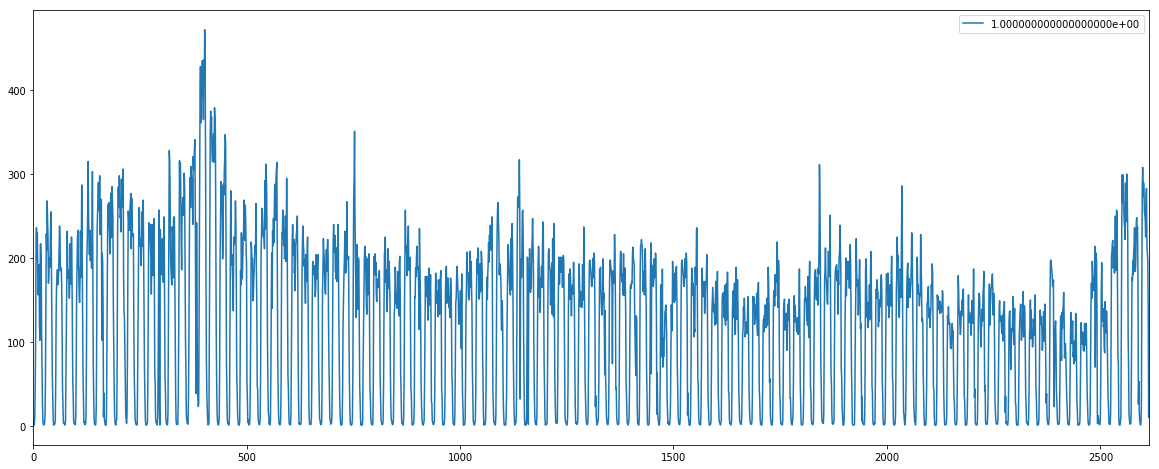
\includegraphics[scale=0.36]{D4D_data_plot}
\caption{Plot for the D4D's dataset.}
\end{figure}

The D4D dataset is divided in two parts: the first 109 days are inserted in TR (training set) this is 2616 hourly samples, and the last 20 days or 480 hourly samples are inserted in TS (testing set).

ACD stands for an Automatic Calls Distribution (ACD) software. Data collected in 2019 from the 1st of January to the 31th of December. Here we have incoming calls information for a technical support. Dataset description could be found in Table 2.
\begin{table}[h!]
\label{tab:table2}
\begin{tabular}{l|l}
name & description \\
\hline
ts1 & Number of hourly received calls by the call center \\
ts2 & Number of hourly handled calls by all the operators in the call center \\
ts3 & Number of hourly answered calls by all the operators in the call center \\
ts4 & Number of hourly routed or queued per operator \\
ts5 & Number of hourly received calls by satisfying \\
ts6 & Hour of the day to which this CDR refers \\
ts7 & Day of the week to which this CDR refers \\
\hline
\end{tabular}
\caption{Fields description for the ACD dataset.}
\end{table}


\begin{figure}
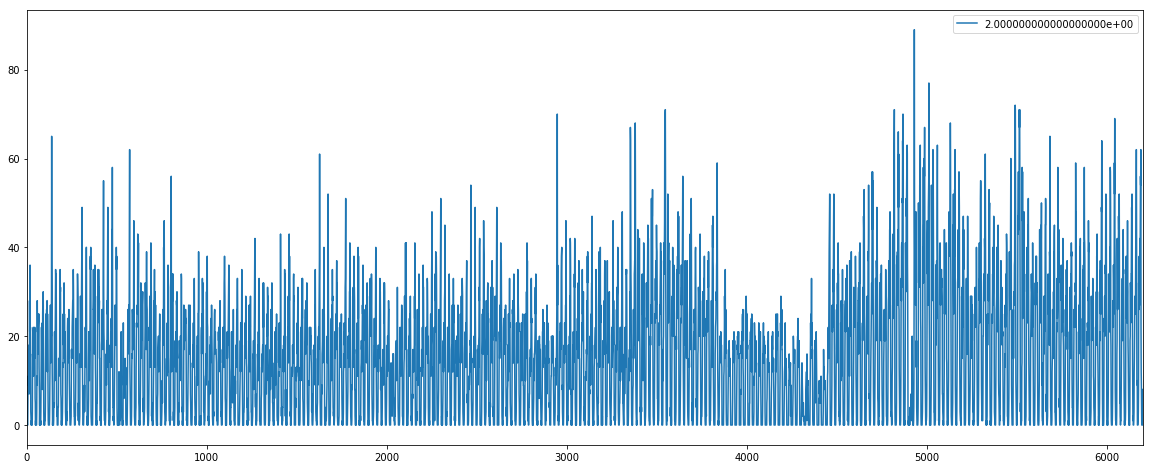
\includegraphics[scale=0.36]{ACD_data_plot}
\caption{Plot for the ACD's dataset.}
\end{figure}

The ACD dataset is divided in two parts: the first 258 days are inserted in TR (training set) this is 6192 hourly samples, and the last 45 days or 1080 hourly samples are inserted in TS (testing set).

SF is a set of incoming calls to the police department in San Francisco. This is the biggest dataset we have, it contains information starting from March 2016 until July 2019.Dataset description could be found in Table 3.
\begin{table}[h!]
\label{tab:table3}
\begin{tabular}{l|l}
name & description \\
\hline
ts1 & Number of hourly received calls by the call center \\
ts2 & Number of hourly received calls belonging to category Passing Call \\
ts3 & Number of hourly received calls belonging to category Traffic Stop \\
ts4 & Number of hourly received calls belonging to other categories \\
ts5 & Hour of the day to which this CDR refers \\
ts6 & Day of the week to which this CDR refers \\
\hline
\end{tabular}
\caption{Fields description for the SF dataset.}
\end{table}

\begin{figure}
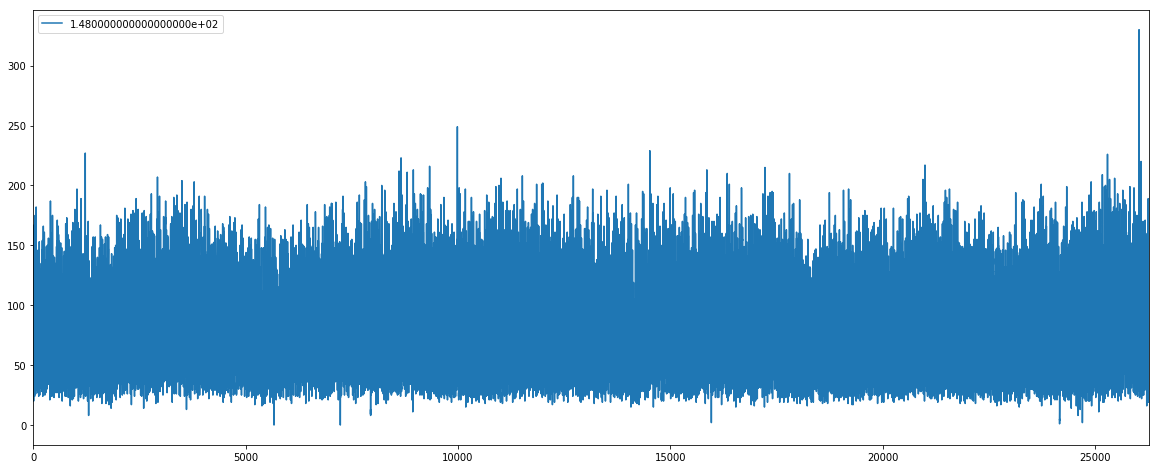
\includegraphics[scale=0.36]{SF_data_plot}
\caption{Plot for the SF's dataset.}
\end{figure}

The SF dataset is divided in two parts: the first 1095 days are inserted in TR (training set) this is 26280 hourly samples, and the last 193 days or 4632 hourly samples are inserted in TS (testing set).

\subsection{Performance measure}

Like in all previous studies here we use the \textit{Normalized Root Mean Squared Error} (NRMSE) for quality check. Using following formula:
\begin{equation}
NRMSE(\widehat{y}, y) = \frac{\sqrt{\frac{1}{n} \sum_{i = 0}^n \left( \widehat{y}_i - y_i \right)^2}}{std(\widehat{y})},
\end{equation}

where $ \widehat{y} $ is the vector of observed values, $ y $ is the vector of predicted ones, $ std(\widehat{y}) $
is the standard deviation of $ \widehat{y} $, and $ n $ is the number of samples of $ \widehat{y} $ and $ y $.

Also the \textit{daily Mean Absolute Percentage Error} (dMAPE) were calculated as well. Formula here:
\begin{equation}
dMAPE(\widehat{y}, y) = \frac{1}{n} \sum_{i = 0}^n \left| \frac{\widehat{y}_i - y_i}{M(d_i)} \right|
\end{equation}

where $ d_i $ is the day corresponding to observation $ i $, and $ M(d_i) $ is the mean of the
observed values in the $ 24 $ hours associated to $ d_i $ and computed as
\begin{equation}
M(d_i) = \frac{1}{24} \sum_{j\in d_i}\widehat{y}_j.
\end{equation}

\subsection{ARIMA}

For ARIMA realisation we used $ARIMA$ model from $statsmodels.tsa.arima.model$ to built a model on the last $730$ elements from training set with order parameter which is a (p,d,q) input for ARIMA, then were loaded to the prediction algorithm. The realisation is in the second block of code.

\lstset{caption={ARIMA realisation.}}
\begin{lstlisting}
length = len(test)
model = ARIMA(train[-730:], order=(24,0,3))
model_fit = model.fit()
test_pred = model_fit.forecast(length)
\end{lstlisting}

If Exponential Smoothing is a well defined method on its own, the ARIMA algorithm heavily depends on the input parameters and for each dataset they are close but still different. Many tests were performed to find compositions from table 4.
\begin{table}[h!]
\label{tab:table4}
\begin{center}
\begin{tabular}{|l|c|c|c|}
\hline
set name & p & d & q \\
\hline
ACD & 24 & 0 & 3 \\
\hline
D4D & 22 & 0 & 3 \\
\hline
SF & 29 & 0 & 5 \\
\hline
\end{tabular}
\end{center}
\caption{The input parameters for ARIMA models.}
\end{table}

ARIMA's performance in long and short term forecasting are shown in Figures 6 and 7 for the ACD dataset, where the blue line describes original data from the testing dataset and the red line describes ARIMA's predictions. In the long term plot we can see that the algorithm starts to follow a strange pattern with the diminution of amplitude and the structure of the shape starts to simplify. Such behaviour is common for all datasets used in this study. The amplitude's changes for all cases seems independent from previous trends in data and the amplitude always lowers.

In the tables 5-10 we can see obtained coefficients in training session:

\newpage

\begin{table}[h!]
\label{tab:table5}
\begin{center}
\begin{tabular}{|l|c|c|c|}
\hline
 & coef  &  std err \\
\hline
const     &    19.9490    &  2.476 \\
\hline
ar.L1     &     0.4868    &  0.255 \\
\hline
ar.L2     &     0.5303   &   0.351 \\
\hline
ar.L3     &    -0.6463    &  0.198 \\
\hline
ar.L4     &     0.0305    &  0.076 \\
\hline
ar.L5     &     0.1633   &   0.080 \\
\hline
ar.L6     &    -0.0544  &    0.054 \\
\hline
ar.L7     &    0.0008  &    0.055 \\
\hline
ar.L8     &     0.0295     & 0.061 \\
\hline
ar.L9     &    -0.0655    &  0.058 \\
\hline
ar.L10    &    0.0053   &   0.057 \\
\hline
ar.L11    &     0.0155 &     0.061 \\
\hline
ar.L12    &    -0.0328     & 0.060 \\
\hline
ar.L13    &    -0.0122    &  0.065 \\
\hline
ar.L14    &     -0.0018  &    0.068 \\
\hline
ar.L15    &    0.0140   &   0.068 \\
\hline
ar.L16    &    0.0263  &    0.072 \\
\hline
ar.L17    &     -0.0425  &    0.073 \\
\hline
ar.L18    &    -0.0459  &    0.071 \\
\hline
ar.L19    &    0.0465  &    0.062 \\
\hline
ar.L20    &    -0.0131   &   0.063 \\
\hline
\end{tabular}
\end{center}
\caption{The coefficients for ARIMA models for the ACD dataset. Part 1}
\end{table}

\begin{table}[h!]
\label{tab:table6}
\begin{center}
\begin{tabular}{|l|c|c|c|}
\hline
 & coef  &  std err \\
\hline
ar.L21    &    -0.0536     & 0.063 \\
\hline
ar.L22    &     0.1274     & 0.048 \\
\hline
ar.L23    &     0.2004    &  0.071 \\
\hline
ar.L24    &     0.1423   &   0.057 \\
\hline
ma.L1     &    -0.1539     & 0.255 \\
\hline
ma.L2     &    -0.2906    &  0.276 \\
\hline
ma.L3     &     0.4476   &   0.162 \\
\hline
sigma2    &    36.7090  &    1.457 \\
\hline
\end{tabular}
\end{center}
\caption{The coefficients for ARIMA models for the ACD dataset. Part 2}
\end{table}

\newpage

\begin{table}[h!]
\label{tab:table7}
\begin{center}
\begin{tabular}{|l|c|c|c|}
\hline
 & coef  &  std err \\
\hline
const     &    103.3240  &  133.909 \\
\hline
ar.L1     &     1.0975  &    0.087 \\
\hline
ar.L2     &     0.2748     & 0.083 \\
\hline
ar.L3     &    -1.0751    &  0.103 \\
\hline
ar.L4     &     0.6461   &   0.090 \\
\hline
ar.L5     &     -0.1120    &  0.072 \\
\hline
ar.L6     &    -0.1228    &  0.087 \\
\hline
ar.L7     &    0.1428    &  0.097 \\
\hline
ar.L8     &     0.0629  &    0.076 \\
\hline
ar.L9     &    -0.2839 &     0.088 \\
\hline
ar.L10    &    0.1306 &     0.093 \\
\hline
ar.L11    &     0.1762     & 0.090 \\
\hline
ar.L12    &    -0.0833    &  0.091 \\
\hline
ar.L13    &    -0.0427   &   0.099 \\
\hline
ar.L14    &     -0.0927 &     0.090 \\
\hline
ar.L15    &    0.0058  &    0.084 \\
\hline
ar.L16    &    0.1338 &     0.087 \\
\hline
ar.L17    &     0.0577     & 0.089 \\
\hline
ar.L18    &    -0.2358    &  0.080 \\
\hline
ar.L19    &    0.1543    &  0.090 \\
\hline
ar.L20    &    0.0071   &   0.076 \\
\hline
\end{tabular}
\end{center}
\caption{The coefficients for ARIMA models for the D4D dataset. Part 1}
\end{table}

\begin{table}[h!]
\label{tab:table8}
\begin{center}
\begin{tabular}{|l|c|c|c|}
\hline
 & coef  &  std err \\
\hline
ar.L21    &    -0.0999 &     0.068 \\
\hline
ar.L22    &     0.2556    &  0.060 \\
\hline
ma.L1     &    -0.3573     & 0.087 \\
\hline
ma.L2     &    -0.6543    &  0.053 \\
\hline
ma.L3     &     0.6628   &   0.068 \\
\hline
sigma2    &    651.2424 &    27.979 \\
\hline
\end{tabular}
\end{center}
\caption{The coefficients for ARIMA models for the D4D dataset. Part 2}
\end{table}

\newpage

\begin{table}[h!]
\label{tab:table9}
\begin{center}
\begin{tabular}{|l|c|c|c|}
\hline
 & coef  &  std err \\
\hline
const     &    97.2010   &   1.145 \\
\hline
ar.L1     &     -0.0372    &  0.330 \\
\hline
ar.L2     &     0.2501    &  0.320 \\
\hline
ar.L3     &    -0.2692   &   0.137 \\
\hline
ar.L4     &     0.3640  &    0.154 \\
\hline
ar.L5     &     0.3718 &     0.212 \\
\hline
ar.L6     &    -0.2422     & 0.102 \\
\hline
ar.L7     &    -0.0596    &  0.052 \\
\hline
ar.L8     &     -0.0202    &  0.056 \\
\hline
ar.L9     &    0.0395     & 0.058 \\
\hline
ar.L10    &    -0.0083   &   0.059 \\
\hline
ar.L11    &     -0.0720    &  0.060 \\
\hline
ar.L12    &    -0.0791    &  0.058 \\
\hline
ar.L13    &    -0.0926   &   0.062 \\
\hline
ar.L14    &     -0.0054 &     0.063 \\
\hline
ar.L15    &    0.0347  &    0.062 \\
\hline
ar.L16    &    -0.0253    &  0.054 \\
\hline
ar.L17    &     0.0136   &   0.054 \\
\hline
ar.L18    &    0.0263   &   0.057 \\
\hline
ar.L19    &    -0.1336     & 0.049 \\
\hline
ar.L20    &    -0.0199    &  0.060 \\
\hline
\end{tabular}
\end{center}
\caption{The coefficients for ARIMA models for the SF dataset. Part 1}
\end{table}

\begin{table}[h!]
\label{tab:table10}
\begin{center}
\begin{tabular}{|l|c|c|c|}
\hline
 & coef  &  std err \\
\hline
ar.L21    &    -0.0128     & 0.060 \\
\hline
ar.L22    &     0.0212    &  0.051 \\
\hline
ar.L23    &     0.1954   &   0.049 \\
\hline
ar.L24    &     0.3894  &    0.073 \\
\hline
ar.L25    &     0.1869     & 0.109 \\
\hline
ar.L26    &     0.0008    &  0.102 \\
\hline
ar.L27    &    -0.1542   &   0.084 \\
\hline
ar.L28    &    -0.1670     & 0.091 \\
\hline
ar.L29    &    -0.1749    &  0.069 \\
\hline
ma.L1     &    0.4563    &  0.333 \\
\hline
ma.L2     &    -0.0044  &    0.280 \\
\hline
ma.L3     &     0.3261 &     0.167 \\
\hline
ma.L4     &    -0.2481    &  0.175 \\
\hline
ma.L5     &    -0.5165    &  0.208 \\
\hline
sigma2    &    278.2435  &    9.611 \\
\hline
\end{tabular}
\end{center}
\caption{The coefficients for ARIMA models for the SF dataset. Part 2}
\end{table}

\newpage

\begin{figure}
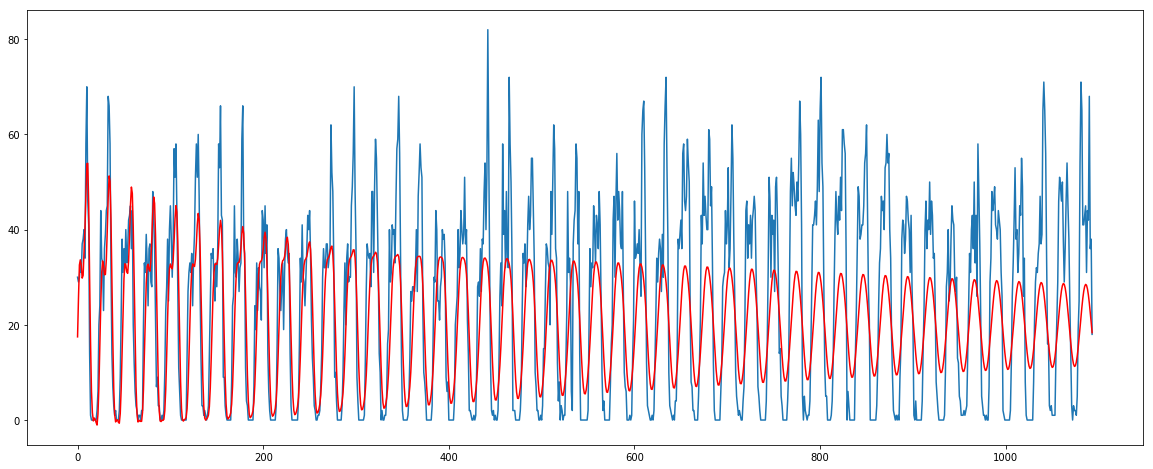
\includegraphics[scale=0.36]{ACD_ARIMA_long_plot}
\caption{Long term ARIMA forecast for the ACD.}
\end{figure}

\begin{figure}
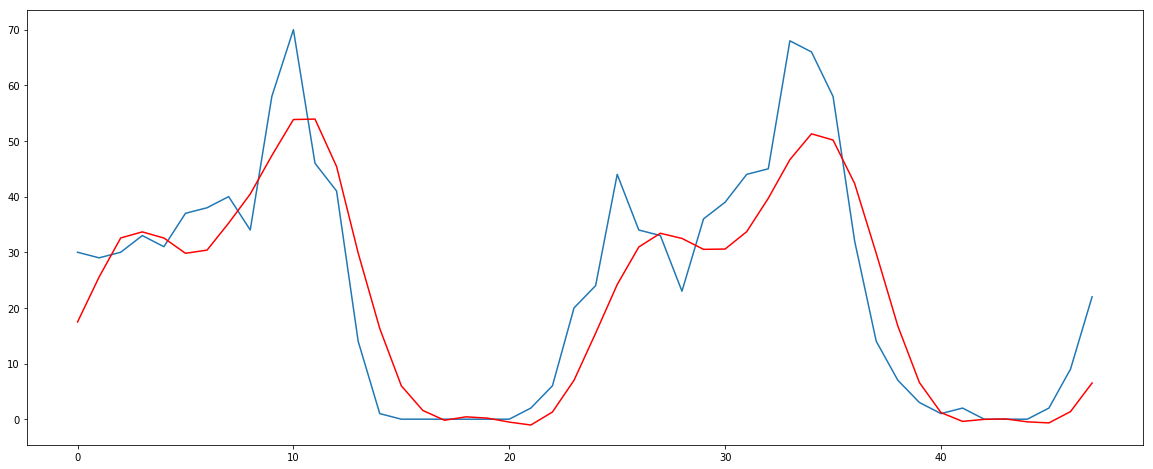
\includegraphics[scale=0.36]{ACD_ARIMA_short_plot}
\caption{ARIMA forecast for the ACD for 48 hours.}
\end{figure}

\subsection{Exponential Smoothing}

For Exponential Smoothing realisation were used $ExponentialSmoothing$ model from $statsmodels.tsa.holtwinters$ to built a model on the last $730$ elements from training set with $seasonal\_periods$ parameter set to $24$ and $seasonal$ parameter is additive, it also could be multiplicative but in this case additive is used, and then were loaded to the prediction algorithm. The realisation is in the third block of code.

\lstset{caption={Exponential Smoothing realisation.}}
\begin{lstlisting}
length = len(test)
model = ExponentialSmoothing(train[-730:], seasonal='add', seasonal_periods=24)
model_fit = model.fit()
fcast = model.forecast(length)
\end{lstlisting}

In Figures 8 and 9 we can see long and short term predictions for the ACD dataset with Exponential Smoothing method for forecasting. Here the black line describes original data from the testing dataset and the green line describes predictions for the Exponential Smoothing. This method shows better results in terms of finding and following patterns for a prolonged periods, but Figure 10 shows on another dataset how crucial it can be, there we can find long term forecasting with the same method for D4D dataset. For Exponential Smoothing function in Python if you want to fit your output to something with cycles you need to include parameter which shows how long these periods last. In this study this parameter was set to $24$ and it represents repetitiveness of the pattern from day to day, with bigger input forecast still will repeat the same founded curve with given length for all forecasting period.

\begin{figure}
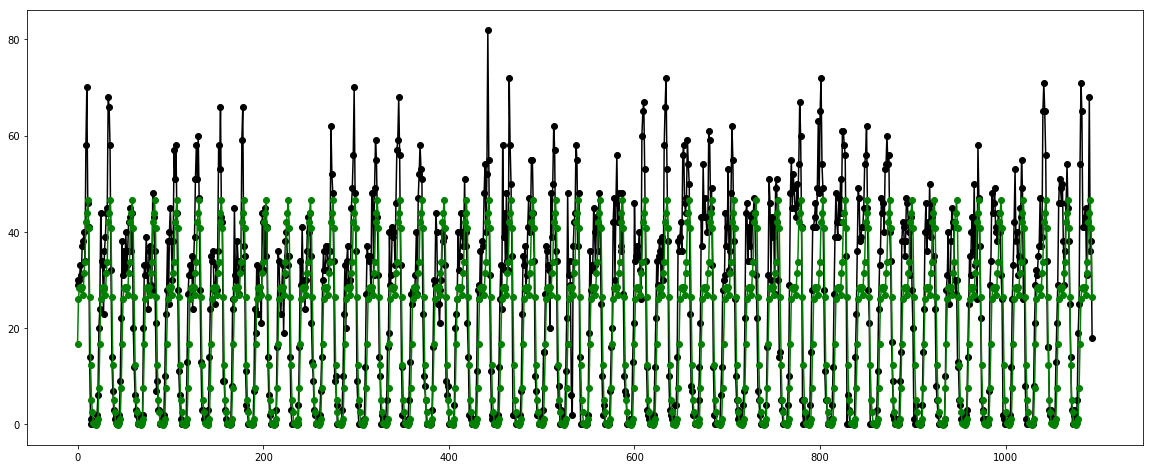
\includegraphics[scale=0.36]{ACD_ES_long_plot}
\caption{Long term Exponential Smoothing forecast for the ACD.}
\end{figure}

\begin{figure}
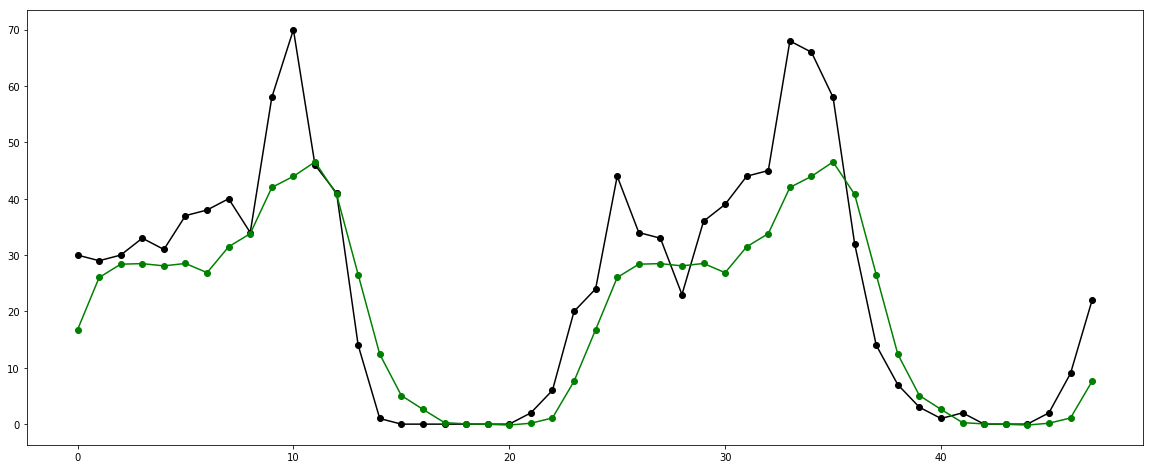
\includegraphics[scale=0.36]{ACD_ES_short_plot}
\caption{Exponential Smoothing forecast for the ACD for 48 hours.}
\end{figure}

\begin{figure}
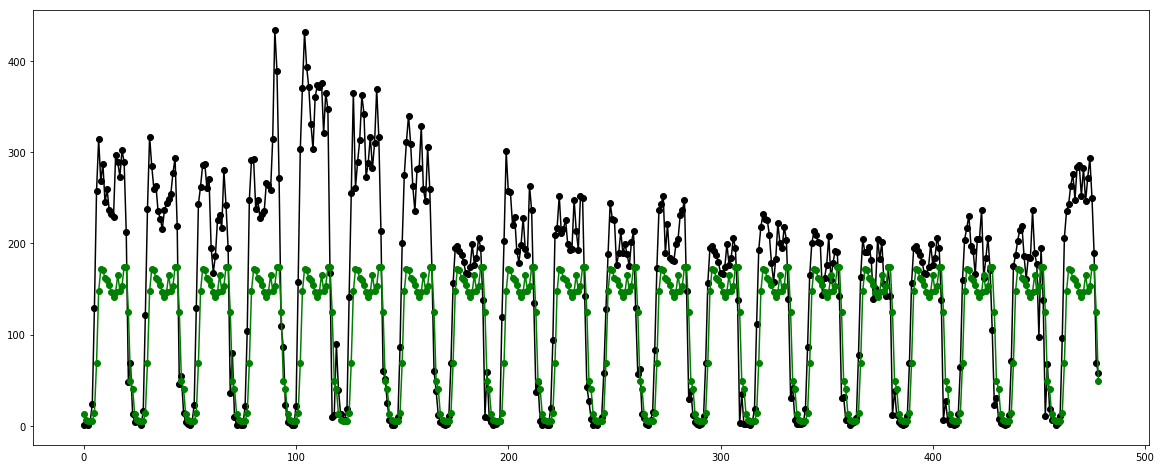
\includegraphics[scale=0.36]{D4D_ES_long_plot}
\caption{Long term Exponential Smoothing forecast for the D4D.}
\end{figure}

\newpage

\section{Results}


The results for all three datasets shown in tables 11-13. For comparison the algorithms from previous study were also used. Here \textit{Echo State Networks} (ESN) \cite{MainPaper}, \textit{Single Layer Feedforward Network} (SLFN) \cite{MainPaper}, \textit{Seasonal Naive} (SN) \cite{SidePaperSN} are all studied before in linked articles.

\begin{table}[h!]
\label{tab:table11}
\begin{center}
\begin{tabular}{l|cc}
D4D & NRMSE & dMAPE \\
\hline
ARIMA & 0.427 & 18.109 \\
ES & 1.414 & 349.645 \\
ESN & 0.3769 & 17.60 \\
SLFN & \textbf{0.3691} & \textbf{16.75} \\
SN & 0.3909 & 17.82 \\
\hline
\end{tabular}
\end{center}
\caption{Comparison results for D4D.}
\end{table}

\begin{table}[h!]
\label{tab:table12}
\begin{center}
\begin{tabular}{l|cc}
ACD & NRMSE & dMAPE \\
\hline
ARIMA & 0.434 & 23.290 \\
ES & 0.625 & 48.095 \\
ESN & 0.3834 & 21.49 \\
SLFN & \textbf{0.3502} & \textbf{19.28} \\
SN & 0.4237 & 23.45 \\
\hline
\end{tabular}
\end{center}
\caption{Comparison results for ACD.}
\end{table}

\begin{table}[h!]
\label{tab:table13}
\begin{center}
\begin{tabular}{l|cc}
SF & NRMSE & dMAPE \\
\hline
ARIMA & 0.560 & 11.705 \\
ES & 0.625 & 48.095 \\
ESN & 0.3775 & 12.60 \\
SLFN & \textbf{0.3582} & \textbf{11.97} \\
SN & 0.4808 & 16.00 \\
\hline
\end{tabular}
\end{center}
\caption{Comparison results for SF.}
\end{table}

Here we can see that the algorithms studied in this work in terms of quality are not as good as research conducted prior, but they demonstrated interesting results. For example ARIMA showed comparable accuracy in short term predictions and Exponential Smoothing (ES) founded base pattern and drew it for the whole prediction period that could be useful to subtract repeated for every day pattern and then study new set of data with only outliers and not basic patterns. Both algorithms showed low performance with full training set loaded, so this results were obtained on 730 hourly samples (number was found in heuristic way). This leads us to computational time for all predictions were calculated in less then 5 minutes. For the ARIMA model with short term predictions with no outliers were to be expected it has a chance to compete with better performing algorithms due to its "easy to built, easy to use" conditions and execution time. 

Downsides: the ARIMA model completely failed in building long term predictions, it has shown some kind of degradation over time both in complexity of the structure for forecasting and in showing repeated trend which implies for all given data. Exponential Smoothing, although it found basic pattern but when it comes to adapting constantly changing conditions it shows inefficient results. For ARIMA part, it could be that better input exists to improve the performance, but I didn't find it.

\section{Conclusions}

ARIMA built sufficiently complex and adaptive structures for short time forecasting periods, with close fit for the real world data. For all the data sets, algorithm shows high dependence on autoregressive part of the model. What is not a surprise due to data daily repetitiveness. Integrated and moving average part show less influence on a performance of the models. Such an algorithm is easy to use and fast to built but with low efficiency for long term forecasts.

Exponential Smoothing technique gives more stable result in terms of long time predictions. With this algorithm you have little chance for successful outcome with complex repetitive structures.

Numerical results for one day predictions demonstrate that ARIMA is good at predicting for short periods, but not as good as neural networks, they are very powerful tool when you try to find some hidden patterns in your data. But in terms of running time to achieve the goal, algorithms from this study are giving more promising run time results.

Both algorithms showed advanced results with ARIMA could even be considered for fast analysis over building neural networks, but for efficiency, previous algorithms showed better results.

\newpage
\phantomsection
\addcontentsline{toc}{section}{Literature}{}
\begin{thebibliography}{X}

\bibitem{Aksin_2007}
Aksin Z, Armony M, Mehrotra V (2007) The modern call center: A multidisciplinary perspective on operations management research. 
Prod Oper Manag 16(6):665-688

\bibitem{Aldor-Noiman_2009}
Aldor-Noiman S, Feigin PD, Mandelbaum A, et al. (2009) Workload forecasting for a call center: Methodology and a case study.
Ann Appl Stat 3(4):1403-1447

\bibitem{Andrews_and_Cunningham_1995}
Andrews BH, Cunningham SM (1995) Ll bean improves call-center forecasting.
Interfaces 25(6):1-13

\bibitem{Antipov_and_Meade_2002}
Antipov A, Meade N (2002) Forecasting call frequency at a financial services call centre.
J Oper Res Soc 53(9):953-960

\bibitem{Avramidis_2004}
Avramidis AN, Deslauriers A, L'Ecuyer P (2004) Modeling daily arrivals to a telephone call center.
Manage Sci 50(7):896-908

\bibitem{SidePaperSN}
Barrow D, Kourentzes N (2018) The impact of special days in call arrivals forecasting: A neural network approach to modelling special days.
Eur J Oper Res 264(3):967-977

\bibitem{Bianchi_1998}
Bianchi L, Jarrett J, Hanumara RC (1998) Improving forecasting for telemarketing centers by arima modeling with intervention.
Int J Forecasting 14(4):497-504

\bibitem{Brown_2005}
Brown L, Gans N, Mandelbaum A, Sakov A, Shen H, Zeltyn S, Zhao L (2005) Statistical analysis of a telephone call center: A queueing-science perspective.
J Am Stat Assoc 100(469):36-50

\bibitem{Gans_2003}
Gans N, Koole G, Mandelbaum A (2003) Telephone call centers: Tutorial, review, and research prospects.
Manuf Serv Op 5(2):79-141

\bibitem{Garnett_2002}
Garnett O, Mandelbaum A, Reiman M (2002) Designing a call center with impatient customers.
Manuf Serv Op 4(3):208-227

\bibitem{Green_2007}
Green LV, Kolesar PJ, Whitt W (2007) Coping with time-varying demand when setting staffing requirements for a service system.
Prod Oper Manag 16(1):13-39

\bibitem{Ibrahim_and_LEcuyer_2013}
Ibrahim R, L'Ecuyer P (2013) Forecasting call center arrivals: Fixed-effects, mixed-effects, and bivariate models.
Manuf Serv Op 15(1):72-85

\bibitem{Ibrahim_2016}
Ibrahim R, Ye H, LEcuyer P, Shen H (2016) Modeling and forecasting call center arrivals: A literature survey and a case study. 
Int J Forecasting 32(3):865-874

\bibitem{Jongbloed_and_Koole_2001}
Jongbloed G, Koole G (2001) Managing uncertainty in call centres using poisson mixtures.
Appl Stoch Model Bus 17(4):307-318

\bibitem{Liao_2012}
Liao S, Koole G, Van Delft C, Jouini O (2012) Staffing a call center with uncertain non-stationary arrival rate and  flexibility.
OR spectrum 34(3):691-721

\bibitem{MainPaper}
Manno A, Rossi F, Smriglio S, Cerone L (2020) Comparing deep and shallow neural networks in forecasting call center arrivals.
https://www.researchsquare.com/article/rs-670306/v1.pdf

\bibitem{MainBook}
Montgomery. Douglas C.(2008) Introduction to time series analysis and forecasting I Douglas C. Montgomery. Cheryl L. Jennings, Murat Kulahci. p. em. - (Wiley series in probability and statistics) Includes bibliographical references and index.
ISBN 978-0-4 71-65397-4 (cloth)

\bibitem{Steckley_2005}
Steckley SG, Henderson SG, Mehrotra V (2005) Performance measures for service systems with a random arrival rate.
In: Proceedings of the Winter Simulation Conference, 2005., IEEE

\bibitem{Taylor_2008}
Taylor JW (2008) Exponentially weighted information criteria for selecting among forecasting models.
Int J Forecasting 24(3):513-524

\bibitem{Taylor_2010}
Taylor JW (2010) Exponentially weighted methods for forecasting intraday time series with multiple seasonal cycles.
Int J Forecasting 26(4):627-646

\bibitem{Wallace_and_Whitt_2005}
Wallace RB, Whitt W (2005) A staffing algorithm for call centers with skill-based routing.
Manuf Serv Op 7(4):276-294

\end{thebibliography}

\end{document}
